\documentclass{article}
\usepackage[margin=1.5cm]{geometry}
\usepackage[parfill]{parskip}
\usepackage[utf8]{inputenc}
\usepackage{amsmath,amssymb,amsfonts,amsthm}
\usepackage{graphicx, hyperref}
\author{Zaccarie Kanit}
\date{22/07/2025}

\title{Probing Security}

\usepackage{filecontents}

\begin{filecontents}{lecture-tum-aci-ss2025-U1.bib}
@inproceedings{DBLP:conf/crypto/IshaiSW03,
  author       = {Yuval Ishai and
                  Amit Sahai and
                  David A. Wagner},
  editor       = {Dan Boneh},
  title        = {Private Circuits: Securing Hardware against Probing Attacks},
  booktitle    = {Advances in Cryptology - {CRYPTO} 2003, 23rd Annual International
                  Cryptology Conference, Santa Barbara, California, USA, August 17-21,
                  2003, Proceedings},
  series       = {Lecture Notes in Computer Science},
  volume       = {2729},
  pages        = {463--481},
  publisher    = {Springer},
  year         = {2003},
  url          = {https://people.eecs.berkeley.edu/~daw/papers/privcirc-crypto03.pdf},
  doi          = {10.1007/978-3-540-45146-4\_27},
}
@inproceedings{DBLP:conf/crypto/BelaidCPRT20,
  author       = {Sonia Belaïd and
                  Jean-Sébastien Coron and
                  Emmanuel Prouff and
                  Matthieu Rivain and
                  Abdul Rahman Taleb},
  editor       = {Daniele Micciancio and
                  Thomas Ristenpart},
  title        = {Random Probing Security: Verification, Composition, Expansion and
                  New Constructions},
  booktitle    = {Advances in Cryptology - {CRYPTO} 2020 - 40th Annual International
                  Cryptology Conference, {CRYPTO} 2020, Santa Barbara, CA, USA, August
                  17-21, 2020, Proceedings, Part {I}},
  series       = {Lecture Notes in Computer Science},
  volume       = {12170},
  pages        = {339--368},
  publisher    = {Springer},
  year         = {2020},
  url          = {https://eprint.iacr.org/2020/786.pdf},
  doi          = {10.1007/978-3-030-56784-2\_12},
}
@misc{vraps,
  title = {VRAPS: (V)erifier of (RA)ndom (P)robing (S)ecurity},
  publisher = {GitHub},
  journal = {GitHub repository},
  howpublished = {\url{https://github.com/CryptoExperts/VRAPS}},
  commit = {f8f878032fd6a5b9f9b9da7ff816c9f401bdc47b}
}
\end{filecontents}

\usepackage{biblatex}
\addbibresource{lecture-tum-aci-ss2025-U1.bib}
\nocite{*}

\begin{document}
\maketitle

\section*{Introduction}

VRAPS~\cite{vraps} is a formal verification tool introduced in~\cite{DBLP:conf/crypto/BelaidCPRT20} to verify the probing security of masked implementations. It verifies:

\begin{itemize}
\item $t$-Probing Security (P)
\item $(p, \varepsilon)$-Random Probing (RP)
\item $(t, p, \varepsilon)$-Random Probing Composability (RPC)
\item $(t, f)$-Random Probing Expandability (RPE)
\end{itemize}

\subsection*{Installation}

The tool requires SageMath (\url{https://www.sagemath.org/index.html}) and Python 3 or higher. To perform the installation, clone the VRAPS repository as follows:

\begin{verbatim}
$ git clone https://github.com/CryptoExperts/VRAPS
\end{verbatim}

\subsection*{Usage}\label{sec:usage}
\begin{enumerate}
\item Create a text file which contains a description of the gadget using the VRAPS syntax. For example, create a file \texttt{isw\_mul\_2.sage} that contains a multiplication gadget as follows:  
\begin{verbatim}
#SHARES 2
#IN a b
#RANDOMS r0
#OUT d

c0 = a0 * b0	
d0 = c0 + r0
c1 = a1 * b1
c1 = c1 + r0
tmp = a0 * b1
c1 = c1 + tmp
tmp = a1 * b0
d1 = c1 + tmp
\end{verbatim}
\item Execute the following command to perform the verification in the 1-probing model (P):
\begin{verbatim}
$ sage verif_tool.sage isw_mul_2.sage P -t 1
Reading file...
Gadget with 2 input(s), 1 output(s), 2 share(s)
Total number of intermediate variables : 11
Total number of output variables : 1
Total number of Wires : 21

Gadget is 1-Probing Secure !
\end{verbatim}
\end{enumerate}

\section*{Exercise \#1}

\begin{enumerate}
  \item Create a multiplication gadget for SecAnd (cf. Lecture L2, $d=2$) and provide its description using the VRAPS syntax here;
  \item Verify its security in the t-probing model using the VRAPS tool for $t\in\{1,2\}$, and report the results here;
  \item Draw a graph (circuit) of the multiplication gadget and provide an explanation of the obtained results here.
\end{enumerate}

\subsection*{Response}
\begin{enumerate}
  \item Here is the proposed multiplication gadget for SecAnd:
  \begin{verbatim}
  #SHARES 2
  #IN a b
  #RANDOMS r0
  #OUT c

  # SecAnd multiplication gadget for d=2 shares
  # Input: a = (a0, a1), b = (b0, b1) 
  # Output: c = (c0, c1) where c = a * b (Boolean multiplication/AND)

  # First output share: c0 = a0*b0 + r0
  c0 = a0 * b0
  c0 = c0 + r0

  # Second output share: c1 = a1*b1 + a0*b1 + a1*b0 + r0
  c1 = a1 * b1
  tmp1 = a0 * b1
  c1 = c1 + tmp1
  tmp2 = a1 * b0
  c1 = c1 + tmp2
  c1 = c1 + r0    #should finish wth the masking
  \end{verbatim}
  \item Here are the results of the verification in the 1-probing model (P): \\
  \textit{\# ISSUE WITH THE VRAPS TOOL, I CAN'T GET THE RESULTS. \#}
  \item Here is the graph of the multiplication gadget Figure \ref{fig:secmult_graph}.
  \begin{figure}[hbt]
    \centering
    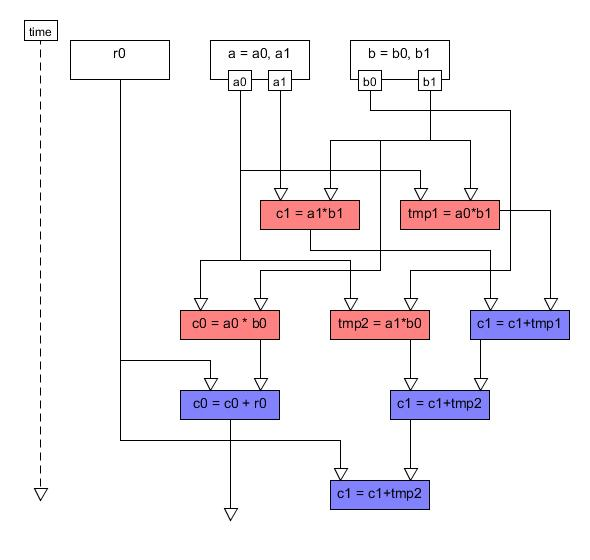
\includegraphics[width=0.45\textwidth]{secmult_graph.jpg}
    \caption{Graph of the SecAnd multiplication gadget}
    \label{fig:secmult_graph}
  \end{figure}
  
\end{enumerate}

\section*{Exercise \#2}

For each of the 3 multiplication gadgets described in \cite[Sec.3, p.11]{DBLP:conf/crypto/BelaidCPRT20}:
\begin{enumerate}
  \item Create a multiplication gadget and provide its description using the VRAPS syntax here;
  \item Verify its security in the t-probing model using the VRAPS tool for $t\in\{1,2\}$, and report the results here;
  \item Draw a graph (circuit) of the multiplication gadget and provide an explanation of the obtained results here.
\end{enumerate}

\subsection*{Response}

\begin{enumerate}
  \item Here are all the proposed multiplication gadgets : 
  \begin{itemize}
    \item ISW-2:
      \begin{verbatim}
        #SHARES 2
        #IN x y
        #RANDOMS r0
        #OUT z
    
        # ISW-2: 2-share ISW multiplication gadget
        # z0 = x0 * y0 + r0
        # z1 = x1 * y1 + r0 + x0 * y1 + x1 * y0
    
        # First share: z0 = x0 * y0 + r0
        z0 = x0 * y0
        z0 = z0 + r0
    
        # Second share: z1 = x1 * y1 + r0 + x0 * y1 + x1 * y0
        z1 = x1 * y1
        z1 = z1 + r0
        tmp1 = x0 * y1
        z1 = z1 + tmp1
        tmp2 = x1 * y0
        z1 = z1 + tmp2
      \end{verbatim}
    \item EC16-3:
      \begin{verbatim}
        #SHARES 3
        #IN x y
        #RANDOMS r0 r1
        #OUT z
        
        # EC16-3: 3-share multiplication gadget from [8]
        # z0 = x0 * y0 + r0 + x0 * y2 + x2 * y0
        # z1 = x1 * y1 + r1 + x0 * y1 + x1 * y0  
        # z2 = x2 * y2 + r0 + r1 + x1 * y2 + x2 * y1
        
        # First share: z0 = x0 * y0 + r0 + x0 * y2 + x2 * y0
        z0 = x0 * y0
        z0 = z0 + r0
        tmp1 = x0 * y2
        z0 = z0 + tmp1
        tmp2 = x2 * y0
        z0 = z0 + tmp2
        
        # Second share: z1 = x1 * y1 + r1 + x0 * y1 + x1 * y0
        z1 = x1 * y1
        z1 = z1 + r1
        tmp3 = x0 * y1
        z1 = z1 + tmp3
        tmp4 = x1 * y0
        z1 = z1 + tmp4
        
        # Third share: z2 = x2 * y2 + r0 + r1 + x1 * y2 + x2 * y1
        z2 = x2 * y2
        z2 = z2 + r0
        z2 = z2 + r1
        tmp5 = x1 * y2
        z2 = z2 + tmp5
        tmp6 = x2 * y1
        z2 = z2 + tmp6
      \end{verbatim}
    \item ISW-3:
      \begin{verbatim}
        #SHARES 3
        #IN x y
        #RANDOMS r0 r1 r2
        #OUT z
        
        # ISW-3: 3-share ISW multiplication gadget
        # z0 = x0 * y0 + r0 + r1
        # z1 = x1 * y0 + (x0 * y1 + r0) + x1 * y1 + r2
        # z2 = x2 * y0 + (x0 * y2 + r1) + (x2 * y1 + (x1 * y2 + r2)) + x2 * y2
        
        # First share: z0 = x0 * y0 + r0 + r1
        z0 = x0 * y0
        z0 = z0 + r0
        z0 = z0 + r1
        
        # Second share: z1 = x1 * y0 + (x0 * y1 + r0) + x1 * y1 + r2
        z1 = x1 * y0
        tmp1 = x0 * y1
        tmp1 = tmp1 + r0
        z1 = z1 + tmp1
        tmp2 = x1 * y1
        z1 = z1 + tmp2
        z1 = z1 + r2
        
        # Third share: z2 = x2 * y0 + (x0 * y2 + r1) + (x2 * y1 + (x1 * y2 + r2)) + x2 * y2
        z2 = x2 * y0
        tmp3 = x0 * y2
        tmp3 = tmp3 + r1
        z2 = z2 + tmp3
        tmp4 = x1 * y2
        tmp4 = tmp4 + r2
        tmp5 = x2 * y1
        tmp5 = tmp5 + tmp4
        z2 = z2 + tmp5
        tmp6 = x2 * y2
        z2 = z2 + tmp6
      \end{verbatim}
  \end{itemize}
\end{enumerate}



\section*{Exercise \#3 (Extra)}
\begin{enumerate}
  \item Provide an explanation why the multiplication gadget of Exercise \#1 is 1-probing secure; alternatively, provide an explanation that
the multiplication gadget described in Sec.~\ref{sec:usage} of this document is 1-probing secure; Hint: see the proof of \cite[Th.
1]{DBLP:conf/crypto/IshaiSW03}.
\end{enumerate}

\subsection*{Response}
\begin{enumerate}
  \item Key Security Properties :
    \begin{itemize}
      \item Fresh Randomness: The random value r0 appears in both output shares, providing masking without correlation to inputs.
      \item Share Independence: Each individual share (a0, a1, b0, b1) is uniformly random and independent of the secret values.
      \item Cross-term Masking: The critical cross-terms (a0b1, a1b0) that could leak information are properly masked by r0.
      \item Uniformity: Any single probe observes either: a uniformly random value, or a combination masked by fresh randomness
    \end{itemize}
\end{enumerate}

\printbibliography

\end{document}

